\documentclass{beamer}
\title{Sleepable RCU in linux}
\usetheme{CambridgeUS}
\usecolortheme{beaver}
\usepackage{makecell}
\usepackage{hyperref}
\usepackage{kotex}
\usepackage{graphics}
\usepackage{booktabs}
\usepackage{listings}
\usepackage{local_dir}
\lstset{inputpath=\rcucode/SRCU/,
  basicstyle=\scriptsize,
  numbers=left,
  xleftmargin=10pt,
  tabsize=2,
  language=C,
}
\graphicspath{ {\rcufigure/SRCU/}}
\author{Chang-Hui Kim}

\begin{document}

\begin{frame}
  \titlepage
\end{frame}

%% -------------------------------------------------------------------------

\section{Intro}

%% recap Caveet RCU background

%% -------------------------------------------------------------------------

\begin{frame}[t]
  \frametitle{Classic RCU}

  \begin{center}
    blocking or sleeping of any sort is strictly prohibited.
  \end{center}

  since arbitrary sleeping in RCU read-side could indefinitely extend grace periods

  \begin{itemize}
  \item in turn could result in arbitrarily large amounts of memory awaiting the end
    of a grace period.
  \item a single read-side critical section could indefinitely delay all RCU callbacks.
  \end{itemize}

\end{frame}

%% -------------------------------------------------------------------------

\begin{frame}[t]
  \frametitle{The problem of \texttt{call\_rcu()}}

  \begin{figure}
    \lstinputlisting[firstline=1, lastline=2]{call_rcu_problem.c}
    \caption{a single thread can generate an arbitrarily large number of
      blocks of memory awaiting a grace period.}
  \end{figure}

  \begin{figure}
    \lstinputlisting[firstline=4, lastline=8]{call_rcu_problem.c}
    \caption{at most a single block of memory per thread awaiting a grace period.}
  \end{figure}
  
\end{frame}

%% -------------------------------------------------------------------------

\begin{frame}[t]
  \frametitle{Implementation Strategy}

  preventing an unbounded number of RCU callbacks.
  \begin{itemize}
  \item refusing to provide asynchronous grace-period interfaces, such as the Classic RCU's \texttt{call\_rcu()} API.
  \item isolating grace-period detection within each subsystem using SRCU.
  \end{itemize}
  
\end{frame}

%% -------------------------------------------------------------------------

\section{API and Usage}

%% -------------------------------------------------------------------------

\begin{frame}[t]
  \frametitle{API list}

  \begin{figure}
    \lstinputlisting[firstline=1, lastline=6]{srcu_implementation.c}
    \caption{SRCU API}
  \end{figure}

  \begin{itemize}
  \item \texttt{call\_rcu()} is removed.
  \item use \texttt{struct srcu\_struct}.
  \end{itemize}
  
\end{frame}

%% -------------------------------------------------------------------------

\begin{frame}[t]
  \frametitle{Read-Side Usage}

  \begin{figure}
    \lstinputlisting[firstline=1, lastline=3]{srcu_usage.c}
    \caption{Read-Side Primitives}
  \end{figure}

  \begin{itemize}
  \item The \texttt{ss} variable is the \texttt{struct srcu\_struct}.
  \item The \texttt{idx} variable is an integer that notifies which grace period this
    read critical section is involved.
  \end{itemize}
  
\end{frame}

%% -------------------------------------------------------------------------

\begin{frame}[t]
  \frametitle{\texttt{idx} Case Study}

  \begin{figure}[ht]
    \centering
    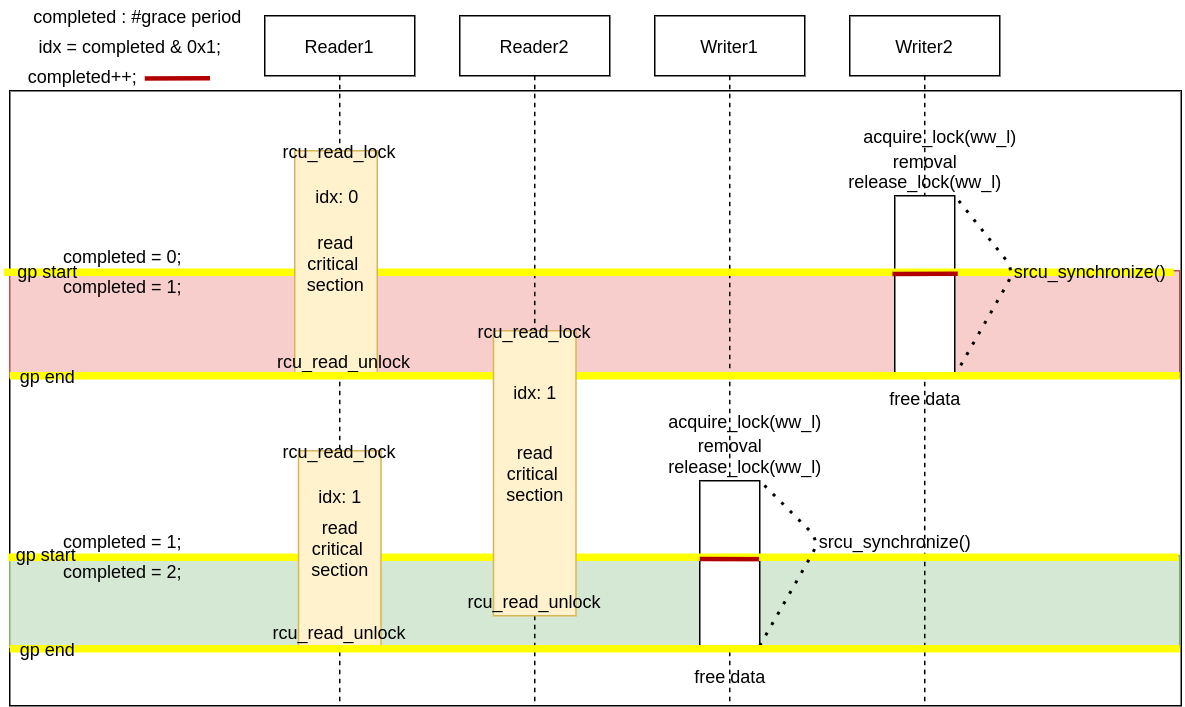
\includegraphics[width=1\textwidth]{idx_example.png}
  \end{figure}
  
\end{frame}

%% -------------------------------------------------------------------------

\begin{frame}[t]
  \frametitle{Update-Side Usage}

  \begin{figure}
    \lstinputlisting[firstline=5, lastline=7]{srcu_usage.c}
    \caption{Update-Side Primitives}
  \end{figure}
  
\end{frame}

%% -------------------------------------------------------------------------

\begin{frame}[t]
  \frametitle{Update-Side Usage}

  \begin{table}
    {\tiny
    \begin{tabular}{c | c | c | c}
      CPU 0 & CPU 1 & CPU 2 & CPU 3\\
      \midrule
      \texttt{i0=srcu\_read\_lock(\&s1);} & & & \texttt{i3=srcu\_read\_lock(\&s2);}\\
      \midrule
      & \makecell{\texttt{synchronize\_srcu(\&s1);} \\ \texttt{[enter]}} & & \\
      \midrule
       & & \texttt{i3=srcu\_read\_lock(\&s1);} & \\
      \midrule
      \texttt{srcu\_read\_unlock(\&s1,i0);} & & & \\
      \midrule
       & \makecell{\texttt{synchroinze\_srcu(\&s1);} \\ \texttt{[exit]}} & & \\
      \midrule
       & & \texttt{srcu\_read\_unlock(\&s1,i2);} & 
    \end{tabular}
    }
    \caption{SRCU Update and Read-Side Critical Sections}
  \end{table}
  
\end{frame}

%% -------------------------------------------------------------------------

\begin{frame}[t]
  \frametitle{Cleanup Example}
  
  \begin{figure}
    \begin{columns}
      \begin{column}{.5\textwidth}
        \lstinputlisting[firstline=9, lastline=23]{srcu_usage.c}
      \end{column}

      \begin{column}{.5\textwidth}
        \lstinputlisting[firstline=25, lastline=31]{srcu_usage.c}
      \end{column}
    \end{columns}
    \caption{SRCU cleanup example}
  \end{figure}
  
\end{frame}

%% -------------------------------------------------------------------------

\section{Implementation}

%% -------------------------------------------------------------------------

\subsection{Data Structures}

%% -------------------------------------------------------------------------

\begin{frame}[t]
  \frametitle{Data Structures}

  \begin{figure}
    \lstinputlisting[firstline=8, lastline=16]{srcu_implementation.c}
  \end{figure}

  \begin{itemize}
  \item \texttt{completed} field is a count of the number of grace periods
    \begin{itemize}
    \item since the \texttt{struct srcu} was initialized.
    \item low-order bit is used to index the \texttt{struct srcu\_struct\_array}.
    \end{itemize}
  \item \texttt{per\_cpu\_ref} field points to the array.
  \item \texttt{mutex} field is used to permit but one \texttt{synchronize\_srcu()} at
    a time to proceed.
  \end{itemize}
  
\end{frame}

%% -------------------------------------------------------------------------

\begin{frame}[t, fragile]
  \frametitle{Data Structures}

  \begin{figure}
    \begin{lstlisting}
      int idx = ss->completed & 0x1; // LSB of completed
      ss->per_cpu_ref[#CPU]->c[idx]++; // array of struct srcu_array
    \end{lstlisting}
    \caption{Pseudo Code Example}
  \end{figure}
  
\end{frame}

%% -------------------------------------------------------------------------

\subsection{Initialization}

%% -------------------------------------------------------------------------

\begin{frame}[t]
  \frametitle{Initialization}

  \begin{figure}
    \lstinputlisting[firstline=18, lastline=24]{srcu_implementation.c}
    \caption{init\_srcu\_struct}
  \end{figure}

  simply initializes \texttt{struct srcu\_struct}'s fields.
  
\end{frame}

%% -------------------------------------------------------------------------

\subsection{Cleanup}

%% -------------------------------------------------------------------------

\begin{frame}[t]
  \frametitle{Count Active Readers}

  \begin{figure}
      \lstinputlisting[firstline=26, lastline=41]{srcu_implementation.c}
    \caption{get the number of active readers.}
  \end{figure}
  
\end{frame}

%% -------------------------------------------------------------------------

\begin{frame}[t]
  \frametitle{Cleanup Function}

  \begin{figure}
      \lstinputlisting[firstline=43, lastline=53]{srcu_implementation.c}
    \caption{cleanup api.}
  \end{figure}

  if the \texttt{sum} is not zero then issues a warning (always bug).
  
\end{frame}

%% -------------------------------------------------------------------------

\subsection{Read-Side}

%% -------------------------------------------------------------------------

\begin{frame}[t]
  \frametitle{Read-Side Implementation}

    \lstinputlisting[firstline=56, lastline=67]{srcu_implementation.c}

  \begin{itemize}
  \item picks up the bottom bit of the grace-period counter. (line 6)
  \item The \texttt{barrier()} is a directive to the compiler that ensures that the index is
    fetched but once. (line 7).
  \item increment the selected counter for the current CPU. (line 8)
  \item in \texttt{CONFIG\_PREEMPT} build, \texttt{srcu\_barrier()} is nop. (line 9)
  \end{itemize}
  
\end{frame}

%% -------------------------------------------------------------------------

\begin{frame}[t]
  \frametitle{Read-Side Implementation}

  \lstinputlisting[firstline=69, lastline=75]{srcu_implementation.c}

  \begin{itemize}
  \item decrement the counter for this CPU.
  \item a given CPU's counters can be observed by other CPUs \textbf{only} in
    cooperation with that CPU's interrupt handlers.
  \end{itemize}
  
\end{frame}

%% -------------------------------------------------------------------------

\subsection{Update-Side Implementation}

%% -------------------------------------------------------------------------

\begin{frame}[t]
  \frametitle{Update-Side Implementation}

  \lstinputlisting[firstline=77, lastline=94]{srcu_implementation.c}

  \begin{itemize}
  \item wait for \texttt{srcu\_read\_lock()}. (line 10, 13)
  \item wait for \texttt{srcu\_read\_unlock()}. (line 16)
  \end{itemize}
  
\end{frame}

%% -------------------------------------------------------------------------

\begin{frame}[t]
  \frametitle{Purpose of \texttt{synchronize\_sched()} (line 10)}

  \begin{columns}
    \begin{column}{.4\textwidth}
      \begin{figure}[ht]
        \centering
        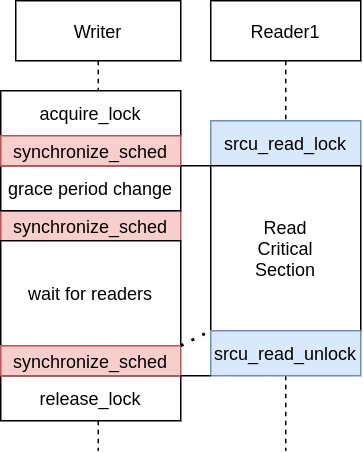
\includegraphics[width=1\textwidth]{synchronize_sched1.png}
        \caption{Inside synchronize\_sched()}
      \end{figure}
    \end{column}

    \begin{column}{.6\textwidth}
      \begin{itemize}
      \item Reader1 sees only changed data. (no old data).
      \item Reader1 will not blocking the next grace period.
      \end{itemize}
    \end{column}
  \end{columns}
  
\end{frame}

%% -------------------------------------------------------------------------

\begin{frame}[t]
  \frametitle{Purpose of \texttt{synchronize\_sched()} (line 13)}

  \begin{columns}
    \begin{column}{.4\textwidth}
      \begin{figure}[ht]
        \centering
        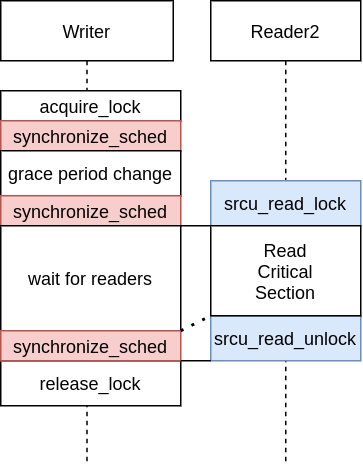
\includegraphics[width=1\textwidth]{synchronize_sched2.png}
      \end{figure}
    \end{column}

    \begin{column}{.6\textwidth}
      \begin{itemize}
      \item wait for any currently-executing \texttt{srcu\_read\_lock} to complete.
      \item after that, all extant instances of \texttt{srcu\_read\_lock} will be using
        the updated value. (\texttt{sp->completed})
      \end{itemize}
    \end{column}
  \end{columns}
  
\end{frame}

%% -------------------------------------------------------------------------

\begin{frame}[t]
  \frametitle{Purpose of \texttt{synchronize\_sched()} (line 16)}

  \begin{columns}
    \begin{column}{.4\textwidth}
      \begin{figure}[ht]
        \centering
        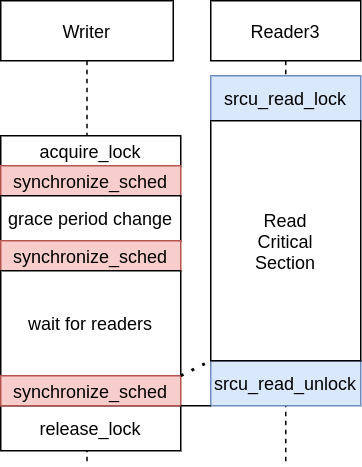
\includegraphics[width=1\textwidth]{synchronize_sched3.png}
      \end{figure}
    \end{column}

    \begin{column}{.6\textwidth}
      \begin{itemize}
      \item Reader3 may sees the old data. (usual case)
      \item wait for \texttt{srcu\_read\_unlock()} completely finish.
      \end{itemize}
    \end{column}
  \end{columns}
  
\end{frame}

%% -------------------------------------------------------------------------

\begin{frame}[t]
  \frametitle{Reference}
  \href{https://lwn.net/Articles/202847/}{LWN Sleepable RCU by Paul McKenney}
  
\end{frame}

\end{document}
